% answers.tex —— 2009 年·普通高等学校招生考试·天津卷·理科 · 参考答案与详细解析片段
% 由 tools/generate_projects.py 依来源总账自 2009/2009_数学真题_天津理_试题.md + 2009/2009_数学真题_天津理_解析正文.md + 2009/2009_数学真题_天津理_答案要点.md 生成，勿手改（改源 MD 后重跑）


\begin{gktip}
固定候选 PDF 仅含题面，无答案、解析和评分标准，原卷亦未标分值；以下为非官方编者独立推导，官方答案字段为空。题面文字层只作定位，分数、根号与三幅图均以 600 dpi 原页复核。
\end{gktip}

\begin{answer}
\gksolhead{1}{}

\textbf{题目}：

$\mathrm i$ 是虚数单位，$\dfrac{5\mathrm i}{2-\mathrm i}=$（　）

（A）$1+2\mathrm i$

（B）$-1-2\mathrm i$

（C）$1-2\mathrm i$

（D）$-1+2\mathrm i$

\Needspace{4\baselineskip}
\textbf{解析}

\nopagebreak[4]
\[\frac{5\mathrm i}{2-\mathrm i}
=\frac{5\mathrm i(2+\mathrm i)}{5}
=\mathrm i(2+\mathrm i)=-1+2\mathrm i,\]

选 D。

\gkanswer{答案：D。}

\end{answer}
\begin{answer}
\gksolhead{2}{}

\textbf{题目}：

设变量 $x,y$ 满足约束条件 $\begin{cases}x+y\geqslant3,\\ x-y\geqslant-1,\\ 2x-y\leqslant3,\end{cases}$ 则目标函数 $z=2x+3y$ 的最小值为（　）

（A）$6$

（B）$7$

（C）$8$

（D）$23$

\Needspace{4\baselineskip}
\textbf{解析}

\Needspace{5\baselineskip}
可行域顶点为 $(1,2)$、$(2,1)$、$(4,5)$，目标值

\nopagebreak[4]
\[z(1,2)=8,\qquad z(2,1)=7,\qquad z(4,5)=23,\]

最小值为 $7$，选 B。

\gkanswer{答案：B。}

\end{answer}
\begin{answer}
\gksolhead{3}{}

\textbf{题目}：

命题「存在 $x_0\in\mathbf R$，$2^{x_0}\leqslant0$」的否定是（　）

（A）不存在 $x_0\in\mathbf R$，$2^{x_0}>0$

（B）存在 $x_0\in\mathbf R$，$2^{x_0}\geqslant0$

（C）对任意的 $x\in\mathbf R$，$2^x\leqslant0$

（D）对任意的 $x\in\mathbf R$，$2^x>0$

\Needspace{4\baselineskip}
\textbf{解析}

\Needspace{5\baselineskip}
特称命题的否定为全称命题，并把结论取反：

\nopagebreak[4]
\[\neg\left(\exists x_0\in\mathbf R,\ 2^{x_0}\leqslant0\right)
\iff \forall x\in\mathbf R,\ 2^x>0 .\]

选 D。

\gkanswer{答案：D。}

\end{answer}
\begin{answer}
\gksolhead{4}{}

\textbf{题目}：

设函数 $f(x)=\dfrac13x-\ln x$（$x>0$），则 $y=f(x)$（　）

（A）在区间 $\left(\dfrac1e,1\right)$，$(1,\mathrm e)$ 内均有零点

（B）在区间 $\left(\dfrac1e,1\right)$，$(1,\mathrm e)$ 内均无零点

（C）在区间 $\left(\dfrac1e,1\right)$ 内有零点，在区间 $(1,\mathrm e)$ 内无零点

（D）在区间 $\left(\dfrac1e,1\right)$ 内无零点，在区间 $(1,\mathrm e)$ 内有零点

\Needspace{4\baselineskip}
\textbf{解析}

\nopagebreak[4]
\[f'(x)=\frac13-\frac1x=\frac{x-3}{3x}.\]

\Needspace{5\baselineskip}
故 $f$ 在 $(0,3)$ 上递减、在 $(3,+\infty)$ 上递增，且

\nopagebreak[4]
\[f(3)=1-\ln3<0 .\]

又 $x\to0^+$ 与 $x\to+\infty$ 时 $f\to+\infty$，故 $f$ 在 $(0,3)$ 与 $(3,+\infty)$ 内各有一个零点。

\Needspace{5\baselineskip}
在 $\left(\frac1e,1\right)$ 上 $f$ 递减且 $f(1)=\frac13>0$，无零点；在 $(1,\mathrm e)$ 上

\nopagebreak[4]
\[f(1)=\frac13>0,\qquad f(\mathrm e)=\frac{\mathrm e}{3}-1<0,\]

有零点。选 D。

\gkanswer{答案：D。}

\end{answer}
\begin{answer}
\gksolhead{5}{}

\textbf{题目}：

阅读如图的程序框图，则输出的 $S=$（　）
\nopagebreak[4]
\begin{center}% 2009 年天津卷理科第 5 题：求 S=2+5+8+11+14 的程序框图。
% 来源 PDF：普通高考/2009/2009天津理.pdf，SHA256 ea758271e47ecf0aadf9b6ea943bcdf2df78b8bf284c3ef26b72c4b69eeb3e80
% 原页：第 1 页（A3 三栏）第 1 栏下部，印刷页 561。
% 重绘依据：开始 → S=0,i=1 → T=3i-1 → S=S+T → i=i+1 → 判断 i>5；否（右）回到 T=3i-1，
%   是（下）→ 输出 S → 结束。
\begin{tikzpicture}[scale=0.9, semithick, >=Stealth,
  node distance=5mm, every node/.style={inner sep=3pt, font=\small}]
  \node (start) [draw, rounded corners=4pt, minimum width=2.0cm, minimum height=0.65cm] {开始};
  \node (init) [draw, minimum width=3.2cm, minimum height=0.65cm, below=of start] {$S=0,\ i=1$};
  \node (t) [draw, minimum width=3.2cm, minimum height=0.65cm, below=of init] {$T=3i-1$};
  \node (add) [draw, minimum width=3.2cm, minimum height=0.65cm, below=of t] {$S=S+T$};
  \node (inc) [draw, minimum width=3.2cm, minimum height=0.65cm, below=of add] {$i=i+1$};
  \node (cond) [draw, diamond, aspect=2.0, minimum width=3.0cm, minimum height=1.0cm, below=of inc] {$i>5$};
  \node (out) [draw, trapezium, trapezium left angle=70, trapezium right angle=110,
    minimum width=2.8cm, minimum height=0.65cm, below=of cond] {输出 $S$};
  \node (end) [draw, rounded corners=4pt, minimum width=2.0cm, minimum height=0.65cm, below=of out] {结束};
  \draw[->] (start) -- (init);
  \draw[->] (init) -- (t);
  \draw[->] (t) -- (add);
  \draw[->] (add) -- (inc);
  \draw[->] (inc) -- (cond);
  \draw[->] (cond) -- (out);
  \node[anchor=west] at ($(cond.south)!0.5!(out.north)+(20pt,-6pt)$) {是};
  \draw[->] (cond.east) -- ++(1.1,0) |- node[pos=0.25, right] {否} (t.east);
  \draw[->] (out) -- (end);
\end{tikzpicture}
\end{center}
\nopagebreak[4]
（A）$26$

（B）$35$

（C）$40$

（D）$57$

\Needspace{4\baselineskip}
\textbf{解析}

\Needspace{5\baselineskip}
循环中 $i=1,2,3,4,5$ 时

\nopagebreak[4]
\[T=3i-1=2,5,8,11,14,\]

\Needspace{5\baselineskip}
累加得

\nopagebreak[4]
\[S=2+5+8+11+14=40 .\]

选 C。

\gkanswer{答案：C。}

\end{answer}
\begin{answer}
\gksolhead{6}{}

\textbf{题目}：

设 $a>0$，$b>0$．若 $\sqrt3$ 是 $3^a$ 与 $3^b$ 的等比中项，则 $\dfrac1a+\dfrac1b$ 的最小值为（　）

（A）$8$

（B）$4$

（C）$1$

（D）$\dfrac14$

\Needspace{4\baselineskip}
\textbf{解析}

\Needspace{5\baselineskip}
$\sqrt3$ 是 $3^a$ 与 $3^b$ 的等比中项：

\nopagebreak[4]
\[(\sqrt3)^2=3^a\cdot3^b=3^{a+b}
\ \Longrightarrow\ a+b=1 .\]

\Needspace{5\baselineskip}
故

\nopagebreak[4]
\[\frac1a+\frac1b=\frac{a+b}{ab}=\frac1{ab}
\geqslant\frac{1}{\left(\frac{a+b}{2}\right)^2}=4,\]

等号在 $a=b=\frac12$ 时成立。选 B。

\gkanswer{答案：B。}

\end{answer}
\begin{answer}
\gksolhead{7}{}

\textbf{题目}：

已知函数 $f(x)=\sin\left(\omega x+\dfrac{\pi}{4}\right)$（$x\in\mathbf R$，$\omega>0$）的最小正周期为 $\pi$．为了得到函数 $g(x)=\cos\omega x$ 的图象，只要将 $y=f(x)$ 的图象（　）

（A）向左平移 $\dfrac{\pi}{8}$ 个单位长度

（B）向右平移 $\dfrac{\pi}{8}$ 个单位长度

（C）向左平移 $\dfrac{\pi}{4}$ 个单位长度

（D）向右平移 $\dfrac{\pi}{4}$ 个单位长度

\Needspace{4\baselineskip}
\textbf{解析}

\Needspace{5\baselineskip}
由周期 $\pi$ 得 $\omega=2$：

\nopagebreak[4]
\[f(x)=\sin\left(2x+\frac\pi4\right),\qquad
g(x)=\cos2x=\sin\left(2x+\frac\pi2\right).\]

\Needspace{5\baselineskip}
左移 $\frac\pi8$：

\nopagebreak[4]
\[f\left(x+\frac\pi8\right)
=\sin\left(2x+\frac\pi4+\frac\pi4\right)
=\sin\left(2x+\frac\pi2\right)=g(x).\]

选 A。

\gkanswer{答案：A。}

\end{answer}
\begin{answer}
\gksolhead{8}{}

\textbf{题目}：

已知函数 $f(x)=\begin{cases}x^2+4x,&x\geqslant0,\\ 4x-x^2,&x<0.\end{cases}$ 若 $f(2-a^2)>f(a)$，则实数 $a$ 的取值范围是（　）

（A）$(-\infty,-1)\cup(2,+\infty)$

（B）$(-1,2)$

（C）$(-2,1)$

（D）$(-\infty,-2)\cup(1,+\infty)$

\Needspace{4\baselineskip}
\textbf{解析}

\Needspace{5\baselineskip}
$x\geqslant0$ 时 $f'=2x+4>0$；$x<0$ 时 $f'=4-2x>0$，且

\nopagebreak[4]
\[f(0^+)=0=f(0^-),\]

\Needspace{5\baselineskip}
故 $f$ 在 $\mathbf R$ 上严格递增。于是

\nopagebreak[4]
\[f(2-a^2)>f(a)\iff 2-a^2>a
\iff a^2+a-2<0
\iff -2<a<1,\]

选 C。

\gkanswer{答案：C。}

\end{answer}
\begin{answer}
\gksolhead{9}{}

\textbf{题目}：

设抛物线 $y^2=2x$ 的焦点为 $F$，过点 $M(\sqrt3,0)$ 的直线与抛物线相交于 $A,B$ 两点，与抛物线的准线相交于 $C$，$|BF|=2$，则 $\triangle BCF$ 与 $\triangle ACF$ 的面积之比 $\dfrac{S_{\triangle BCF}}{S_{\triangle ACF}}=$（　）

（A）$\dfrac45$

（B）$\dfrac23$

（C）$\dfrac47$

（D）$\dfrac12$

\Needspace{4\baselineskip}
\textbf{解析}

$y^2=2x$ 中 $p=\frac12$，焦点 $F\left(\frac12,0\right)$，准线 $x=-\frac12$。

$|BF|=2$ 即 $B$ 到准线的距离为 $2$，故 $x_B=2-\frac12=\frac32$，$y_B^2=3$。

取 $B\left(\frac32,\sqrt3\right)$，直线 $MB$ 与抛物线另一交点为 $A$，计算得 $x_A=2$（由 $y^2=2x$ 与直线方程联立）。$C$ 在准线上，$x_C=-\frac12$。

\Needspace{5\baselineskip}
因 $A,B,C$ 共线，$\triangle BCF$ 与 $\triangle ACF$ 以 $CF$ 为公共底，面积比等于 $B$、$A$ 到直线 $CF$ 的距离比，也就是

\nopagebreak[4]
\[\frac{S_{\triangle BCF}}{S_{\triangle ACF}}
=\frac{|CB|}{|CA|}
=\frac{\frac32+\frac12}{2+\frac12}=\frac{2}{5/2}=\frac45 .\]

选 A。

\gkanswer{答案：A。}

\end{answer}
\begin{answer}
\gksolhead{10}{}

\textbf{题目}：

$0<b<1+a$．若关于 $x$ 的不等式 $(x-b)^2>(ax)^2$ 的解集中的整数恰有 $3$ 个，则（　）

（A）$-1<a<0$

（B）$0<a<1$

（C）$1<a<3$

（D）$3<a<6$

\Needspace{4\baselineskip}
\textbf{解析}

\nopagebreak[4]
\[(x-b)^2>(ax)^2\iff (1-a^2)x^2-2bx+b^2>0 .\]

由 $0<b<1+a$ 知 $a>-1$。

\begin{itemize}
\item $-1<a\leqslant0$：$1-a^2>0$，解集在两根之外，无界，含无穷多整数。
\item $0<a<1$：同样 $1-a^2>0$，解集无界。
\item $a>1$：$1-a^2<0$，抛物线开口向下，解集为两根之间：
\end{itemize}

\nopagebreak[4]
\[\left(\frac{b}{1-a},\ \frac{b}{1+a}\right).\]

\Needspace{5\baselineskip}
右端点 $\frac{b}{1+a}\in(0,1)$，故区间内整数自某个负整数到 $0$。恰有 $3$ 个整数时为 $\{-2,-1,0\}$，需

\nopagebreak[4]
\[-3\leqslant\frac{b}{1-a}<-2
\iff 2<\frac{b}{a-1}\leqslant3 .\]

\Needspace{5\baselineskip}
存在 $b\in(0,1+a)$ 满足此式，等价于 $\left(2(a-1),3(a-1)\right]$ 与 $(0,1+a)$ 有公共部分，即

\nopagebreak[4]
\[2(a-1)<1+a\iff a<3 .\]

\Needspace{5\baselineskip}
结合 $a>1$ 得

\nopagebreak[4]
\[1<a<3,\]

选 C。

\gkanswer{答案：C。}

\end{answer}
\begin{answer}
\gksolhead{11}{}

\textbf{题目}：

某学院的 $A,B,C$ 三个专业共有 $1200$ 名学生，为了调查这些学生勤工俭学的情况，拟采用分层抽样的方法抽取一个容量为 $120$ 的样本．已知该学院的 $A$ 专业有 $380$ 名学生，$B$ 专业有 $420$ 名学生，则在该学院的 $C$ 专业应抽取\gkblank{}名学生．

\Needspace{4\baselineskip}
\textbf{解析}

\Needspace{5\baselineskip}
$C$ 专业有 $1200-380-420=400$ 名学生，抽样比

\nopagebreak[4]
\[\frac{120}{1200}=\frac1{10},\]

故应抽取 $400\times\frac1{10}=40$ 名。

\gkanswer{答案：$40$。}

\end{answer}
\begin{answer}
\gksolhead{12}{}

\textbf{题目}：

如图是一个几何体的三视图，若它的体积是 $3\sqrt3$，则 $a=$\gkblank{}．
\nopagebreak[4]
\begin{center}% 2009 年天津卷理科第 12 题：直三棱柱的三视图。
% 来源 PDF：普通高考/2009/2009天津理.pdf，SHA256 ea758271e47ecf0aadf9b6ea943bcdf2df78b8bf284c3ef26b72c4b69eeb3e80
% 原页：第 1 页（A3 三栏）第 2 栏中部，印刷页 561。
% 重绘依据：正视图为 3×a 矩形；侧视图为底边 2、高 a 的三角形；俯视图为 3×2 矩形，
%   中间一条平行于长的实线把深度分成 1 与 1 两段；尺寸与标注按原图。
\begin{tikzpicture}[scale=0.95, semithick, every node/.style={inner sep=1.2pt}]
  % 正视图
  \draw (0,1.5) rectangle (3,3.0);
  \node[anchor=east] at (-0.1,2.25) {$a$};
  \node[anchor=north] at (1.5,1.35) {正视图};
  % 侧视图
  \draw (4.2,1.5) -- (5.8,1.5) -- (5.0,3.0) -- cycle;
  \node[anchor=north] at (5.0,1.05) {侧视图};
  \node[anchor=north] at (5.0,1.32) {$2$};
  % 俯视图
  \draw (0,-0.35) rectangle (3,0.65);
  \draw (0,0.15) -- (3,0.15);
  \node[anchor=north] at (1.5,-0.5) {俯视图};
  \node[anchor=east] at (-0.1,-0.1) {$1$};
  \node[anchor=east] at (-0.1,0.4) {$1$};
\end{tikzpicture}
\end{center}
\nopagebreak[4]
\Needspace{4\baselineskip}
\textbf{解析}

\Needspace{5\baselineskip}
由三视图，该几何体是底面为直角三角形（直角边 $3$、$2$）、高为 $a$ 的直三棱柱：

\nopagebreak[4]
\[V=\frac12\cdot3\cdot2\cdot a=3a .\]

由 $V=3\sqrt3$ 得 $a=\sqrt3$。

\gkanswer{答案：$\sqrt3$。}

\end{answer}
\begin{answer}
\gksolhead{13}{}

\textbf{题目}：

设直线 $l_1$ 的参数方程为 $\begin{cases}x=1+t,\\ y=1+3t,\end{cases}$（$t$ 为参数），直线 $l_2$ 的方程为 $y=3x+4$，则 $l_1$ 与 $l_2$ 的距离为\gkblank{}．

\Needspace{4\baselineskip}
\textbf{解析}

\Needspace{5\baselineskip}
$l_1$ 的参数方程消去 $t$：

\nopagebreak[4]
\[t=x-1,\qquad y=1+3(x-1)=3x-2 .\]

\Needspace{5\baselineskip}
故 $l_1\parallel l_2$。两平行线

\nopagebreak[4]
\[3x-y-2=0,\qquad 3x-y+4=0\]

\Needspace{5\baselineskip}
的距离为

\nopagebreak[4]
\[d=\frac{|4-(-2)|}{\sqrt{3^2+(-1)^2}}
=\frac6{\sqrt{10}}=\frac{3\sqrt{10}}{5} .\]

\gkanswer{答案：$\frac{3\sqrt{10}}{5}$。}

\end{answer}
\begin{answer}
\gksolhead{14}{}

\textbf{题目}：

若圆 $x^2+y^2=4$ 与圆 $x^2+y^2+2ay-6=0$（$a>0$）的公共弦的长为 $2\sqrt3$，则 $a=$\gkblank{}．

\Needspace{4\baselineskip}
\textbf{解析}

\Needspace{5\baselineskip}
两圆方程相减得公共弦：

\nopagebreak[4]
\[2ay-6=-4\ \Longrightarrow\ y=\frac1a .\]

\Needspace{5\baselineskip}
圆 $x^2+y^2=4$ 上该弦的半弦长为

\nopagebreak[4]
\[\sqrt{4-\frac1{a^2}}=\sqrt3
\ \Longrightarrow\ \frac1{a^2}=1\ \Longrightarrow\ a=1\ (a>0).\]

\gkanswer{答案：$1$。}

\end{answer}
\begin{answer}
\gksolhead{15}{}

\textbf{题目}：

在四边形 $ABCD$ 中，$\overrightarrow{AB}=\overrightarrow{DC}=(1,1)$，$\dfrac{1}{|\overrightarrow{BA}|}\overrightarrow{BA}+\dfrac{1}{|\overrightarrow{BC}|}\overrightarrow{BC}=\dfrac{\sqrt3}{|\overrightarrow{BD}|}\overrightarrow{BD}$，则四边形 $ABCD$ 的面积为\gkblank{}．

\Needspace{4\baselineskip}
\textbf{解析}

$\overrightarrow{AB}=\overrightarrow{DC}=(1,1)$，故 $ABCD$ 为平行四边形，$AB=BC$ 待定。

\Needspace{5\baselineskip}
记

\nopagebreak[4]
\[\boldsymbol u=\frac{\overrightarrow{BA}}{|\overrightarrow{BA}|},\qquad
\boldsymbol v=\frac{\overrightarrow{BC}}{|\overrightarrow{BC}|},\]

\Needspace{5\baselineskip}
则

\nopagebreak[4]
\[\boldsymbol u+\boldsymbol v=\frac{\sqrt3}{|\overrightarrow{BD}|}\overrightarrow{BD},\]

\Needspace{5\baselineskip}
故

\nopagebreak[4]
\[|\boldsymbol u+\boldsymbol v|=\sqrt3 .\]

\Needspace{5\baselineskip}
设 $\angle ABC=\theta$：

\nopagebreak[4]
\[|\boldsymbol u+\boldsymbol v|=2\cos\frac\theta2=\sqrt3
\ \Longrightarrow\ \theta=60^\circ .\]

\Needspace{5\baselineskip}
又 $\overrightarrow{BD}=\overrightarrow{BA}+\overrightarrow{BC}$ 与 $\boldsymbol u+\boldsymbol v$ 同向，故

\nopagebreak[4]
\[|\overrightarrow{BA}|=|\overrightarrow{BC}|=\sqrt2 .\]

\Needspace{5\baselineskip}
即 $ABCD$ 是边长为 $\sqrt2$、夹角 $60^\circ$ 的菱形，面积

\nopagebreak[4]
\[S=(\sqrt2)^2\sin60^\circ=\sqrt3 .\]

\gkanswer{答案：$\sqrt3$。}

\end{answer}
\begin{answer}
\gksolhead{16}{}

\textbf{题目}：

用数字 $0,1,2,3,4,5,6$ 组成没有重复数字的四位数，其中个位、十位和百位上的数字之和为偶数的四位数共有\gkblank{}个．（用数字作答）

\Needspace{4\baselineskip}
\textbf{解析}

按千位数字分类（数字取自 $0,1,\dots,6$，无重复）。

\begin{itemize}
\item 千位为奇数 $1,3,5$（$3$ 种）：余下 $2$ 个奇数、$4$ 个偶数。后三位和为偶数需取 $0$ 个或 $2$ 个奇数。逐一计数（并排除百位为 $0$）得每个千位 $48$ 个，共 $144$ 个。
\item 千位为非零偶数 $2,4,6$（$3$ 种）：余下 $3$ 个奇数、$3$ 个偶数，每个千位 $60$ 个，共 $180$ 个。
\end{itemize}

\Needspace{5\baselineskip}
合计

\nopagebreak[4]
\[144+180=324 .\]

（穷举 $0$ 至 $6$ 的全部四位无重复数复核，结果一致。）

\gkanswer{答案：$324$。}

\end{answer}
\begin{answer}
\gksolhead{17}{}

\textbf{题目}：

在 $\triangle ABC$ 中，$BC=\sqrt5$，$AC=3$，$\sin C=2\sin A$．

（1）求 $AB$ 的值；

（2）求 $\sin\left(2A-\dfrac{\pi}{4}\right)$ 的值．

\Needspace{4\baselineskip}
\textbf{解析}

\Needspace{5\baselineskip}
（1）由正弦定理

\nopagebreak[4]
\[\frac{AB}{\sin C}=\frac{BC}{\sin A}
\ \Longrightarrow\ AB=BC\cdot\frac{\sin C}{\sin A}=2\sqrt5 .\]

\Needspace{5\baselineskip}
（2）由余弦定理

\nopagebreak[4]
\[\cos A=\frac{AB^2+AC^2-BC^2}{2\cdot AB\cdot AC}
=\frac{20+9-5}{12\sqrt5}=\frac2{\sqrt5},\]

\Needspace{5\baselineskip}
故 $\sin A=\frac1{\sqrt5}$，$\sin2A=\frac45$，$\cos2A=\frac35$。于是

\nopagebreak[4]
\[\sin\left(2A-\frac\pi4\right)
=\frac{\sin2A-\cos2A}{\sqrt2}=\frac{\sqrt2}{10} .\]

\gkanswer{答案：（1）$AB=2\sqrt5$；（2）$\frac{\sqrt2}{10}$。}

\end{answer}
\begin{answer}
\gksolhead{18}{}

\textbf{题目}：

在 $10$ 件产品中，有 $3$ 件一等品，$4$ 件二等品，$3$ 件三等品．从这 $10$ 件产品中任取 $3$ 件，求：

（1）取出的 $3$ 件产品中一等品件数 $X$ 的分布列和数学期望；

（2）取出的 $3$ 件产品中一等品件数多于二等品件数的概率．

\Needspace{4\baselineskip}
\textbf{解析}

\Needspace{5\baselineskip}
（1）$\mathrm C_{10}^3=120$。

\nopagebreak[4]
\[P(X=0)=\frac{\mathrm C_3^0\mathrm C_7^3}{120}=\frac{35}{120}=\frac7{24},\]

\nopagebreak[4]
\[P(X=1)=\frac{\mathrm C_3^1\mathrm C_7^2}{120}=\frac{63}{120}=\frac{21}{40},\]

\nopagebreak[4]
\[P(X=2)=\frac{\mathrm C_3^2\mathrm C_7^1}{120}=\frac{21}{120}=\frac7{40},\]

\nopagebreak[4]
\[P(X=3)=\frac{\mathrm C_3^3\mathrm C_7^0}{120}=\frac1{120}.\]

\nopagebreak[4]
\[EX=\frac{0\cdot35+1\cdot63+2\cdot21+3\cdot1}{120}
=\frac{108}{120}=\frac9{10} .\]

（2）设二等品件数为 $Y$，枚举 $X>Y$ 且 $X+Y\leqslant3$ 的情形：

\begin{itemize}
\item $(X,Y)=(1,0)$：三等品 $2$ 件，$\mathrm C_3^1\mathrm C_3^2=9$；
\item $(2,0)$：三等品 $1$ 件，$\mathrm C_3^2\mathrm C_3^1=9$；
\item $(2,1)$：三等品 $0$ 件，$\mathrm C_3^2\mathrm C_4^1=12$；
\item $(3,0)$：$\mathrm C_3^3=1$。
\end{itemize}

\Needspace{5\baselineskip}
共 $31$ 种，故

\nopagebreak[4]
\[P(X>Y)=\frac{31}{120} .\]

\gkanswer{答案：（1）分布列见下，$EX=\frac9{10}$；（2）$\frac{31}{120}$。}

\end{answer}
\begin{answer}
\gksolhead{19}{}

\textbf{题目}：

如图，在五面体 $ABCDEF$ 中，$FA\perp$ 平面 $ABCD$，$AD\parallel BC\parallel FE$，$AB\perp AD$，$M$ 为 $EC$ 的中点，$AF=AB=BC=FE=\dfrac12AD$．
\nopagebreak[4]
\begin{center}% 2009 年天津卷理科第 19 题：五面体 ABCDEF，FA⊥平面 ABCD，AD∥BC∥FE。
% 来源 PDF：普通高考/2009/2009天津理.pdf，SHA256 ea758271e47ecf0aadf9b6ea943bcdf2df78b8bf284c3ef26b72c4b69eeb3e80
% 原页：第 2 页（A3 三栏）第 1 栏上部，印刷页 562。
% 重绘依据：A 前左下、B 前右下、C 右后、D 左后；F 在 A 正上方，E 在 F 后上方且 FE∥AD；
%   M 为 EC 中点。被遮挡的 D-A 画虚线。
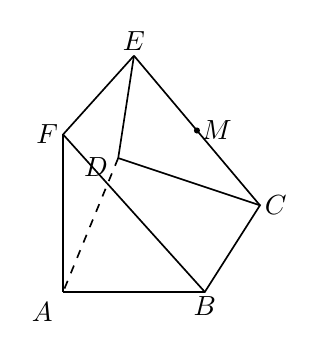
\begin{tikzpicture}[scale=1.0, semithick, every node/.style={inner sep=1.5pt}]
  \coordinate (A) at (0,0);
  \coordinate (B) at (1.8,0);
  \coordinate (C) at (2.5,1.1);
  \coordinate (D) at (0.7,1.7);
  \coordinate (F) at (0,2.0);
  \coordinate (E) at (0.9,3.0);
  \coordinate (M) at (1.7,2.05);
  % 底面
  \draw (A) -- (B) -- (C) -- (D);
  \draw[dashed] (D) -- (A);
  % 棱
  \draw (A) -- (F);
  \draw (F) -- (E);
  \draw (B) -- (F);
  \draw (C) -- (E);
  \draw (E) -- (D);
  % M
  \fill (M) circle (1.1pt);
  \node[anchor=north east] at ([xshift=-2pt,yshift=-2pt]A) {$A$};
  \node[anchor=north] at (B) {$B$};
  \node[anchor=west] at (C) {$C$};
  \node[anchor=north east] at ([xshift=-2pt,yshift=2pt]D) {$D$};
  \node[anchor=east] at (F) {$F$};
  \node[anchor=south] at (E) {$E$};
  \node[anchor=west] at (M) {$M$};
\end{tikzpicture}
\end{center}
\nopagebreak[4]
（1）求异面直线 $BF$ 与 $DE$ 所成的角的大小；

（2）证明平面 $AMD\perp$ 平面 $CDE$；

（3）求二面角 $A-CD-E$ 的余弦值．

\Needspace{4\baselineskip}
\textbf{解析}

\Needspace{5\baselineskip}
设 $AB=1$，则 $AD=2$，$AF=BC=FE=1$。取

\nopagebreak[4]
\[A(0,0,0),\ B(1,0,0),\ D(0,2,0),\ C(1,1,0),\]
\nopagebreak[4]
\[F(0,0,1),\ E(0,1,1),\ M\left(\frac12,1,\frac12\right).\]

\Needspace{5\baselineskip}
（1）

\nopagebreak[4]
\[\overrightarrow{BF}=(-1,0,1),\qquad \overrightarrow{DE}=(0,-1,1),\]

\nopagebreak[4]
\[\cos\theta=\frac{1}{\sqrt2\cdot\sqrt2}=\frac12,\]

故异面直线 $BF$ 与 $DE$ 所成角为 $60^\circ$。

\Needspace{5\baselineskip}
（2）平面 $AMD$：

\nopagebreak[4]
\[\overrightarrow{AM}=\left(\frac12,1,\frac12\right),\qquad
\overrightarrow{AD}=(0,2,0),\]

\nopagebreak[4]
\[\mathbf n_1=\overrightarrow{AM}\times\overrightarrow{AD}=(-1,0,1).\]

\Needspace{5\baselineskip}
平面 $CDE$：

\nopagebreak[4]
\[\overrightarrow{DC}=(1,-1,0),\qquad \overrightarrow{DE}=(0,-1,1),\]

\nopagebreak[4]
\[\mathbf n_2=\overrightarrow{DC}\times\overrightarrow{DE}=(-1,-1,-1).\]

$\mathbf n_1\cdot\mathbf n_2=0$，故平面 $AMD\perp$ 平面 $CDE$。

\Needspace{5\baselineskip}
（3）平面 $ACD$ 即 $z=0$，法向量 $(0,0,1)$；平面 $CDE$ 法向量 $(-1,-1,-1)$。设二面角为 $\theta$：

\nopagebreak[4]
\[\cos\theta=\frac{|(0,0,1)\cdot(-1,-1,-1)|}{\sqrt3}
=\frac{\sqrt3}{3} .\]

\gkanswer{答案：（1）$60^\circ$；（2）证明见解析；（3）$\frac{\sqrt3}{3}$。}

\end{answer}
\begin{answer}
\gksolhead{20}{}

\textbf{题目}：

已知函数 $f(x)=(x^2+ax-2a^2+3a)\mathrm e^x$（$x\in\mathbf R$），其中 $a\in\mathbf R$．

（1）当 $a=0$ 时，求曲线 $y=f(x)$ 在点 $(1,f(1))$ 处的切线的斜率；

（2）当 $a\neq\dfrac23$ 时，求函数 $f(x)$ 的单调区间与极值．

\Needspace{4\baselineskip}
\textbf{解析}

\Needspace{5\baselineskip}
（1）$a=0$：

\nopagebreak[4]
\[f(x)=x^2\mathrm e^x,\qquad f'(x)=(x^2+2x)\mathrm e^x,\]

\nopagebreak[4]
\[f'(1)=3\mathrm e .\]

\Needspace{5\baselineskip}
（2）

\nopagebreak[4]
\[f'(x)=\left[x^2+(a+2)x-2a^2+4a\right]\mathrm e^x
=(x+2a)(x-a+2)\mathrm e^x .\]

两根 $x=-2a$、$x=a-2$。

\begin{itemize}
\item $a>\frac23$ 时 $-2a<a-2$：
\end{itemize}

  增区间 $(-\infty,-2a)$、$(a-2,+\infty)$，减区间 $(-2a,a-2)$；极大值 $f(-2a)$，极小值 $f(a-2)$。

\begin{itemize}
\item $a<\frac23$ 时 $a-2<-2a$：
\end{itemize}

  增区间 $(-\infty,a-2)$、$(-2a,+\infty)$，减区间 $(a-2,-2a)$；极大值 $f(a-2)$，极小值 $f(-2a)$。

\gkanswer{答案：（1）$3\mathrm e$；（2）见下。}

\end{answer}
\begin{answer}
\gksolhead{21}{}

\textbf{题目}：

已知椭圆 $\dfrac{x^2}{a^2}+\dfrac{y^2}{b^2}=1$（$a>b>0$）的两个焦点分别为 $F_1(-c,0)$ 和 $F_2(c,0)$（$c>0$），过点 $E\left(\dfrac{a^2}{c},0\right)$ 的直线与椭圆相交于 $A,B$ 两点，且 $F_1A\parallel F_2B$，$|F_1A|=2|F_2B|$．

（1）求椭圆的离心率；

（2）求直线 $AB$ 的斜率；

（3）设点 $C$ 与点 $A$ 关于坐标原点对称，直线 $F_2B$ 上有一点 $H(m,n)$（$m\neq0$）在 $\triangle AF_1C$ 的外接圆上，求 $\dfrac nm$ 的值．

\Needspace{4\baselineskip}
\textbf{解析}

\Needspace{5\baselineskip}
（1）设 $B(x,y)$，由 $F_1A\parallel F_2B$ 且 $|F_1A|=2|F_2B|$ 取

\nopagebreak[4]
\[\overrightarrow{F_1A}=2\overrightarrow{F_2B},\]

\Needspace{5\baselineskip}
则

\nopagebreak[4]
\[A=(2x-3c,2y).\]

\Needspace{5\baselineskip}
$A,B$ 在椭圆上，两式相减得

\nopagebreak[4]
\[x=\frac{a^2+3c^2}{4c} .\]

\Needspace{5\baselineskip}
又 $A,B,E\left(\frac{a^2}{c},0\right)$ 共线，比较横坐标：

\nopagebreak[4]
\[2x-3c-\frac{a^2}{c}=2\left(x-\frac{a^2}{c}\right)
\ \Longrightarrow\ a^2=3c^2 .\]

\Needspace{5\baselineskip}
故

\nopagebreak[4]
\[e=\frac ca=\frac{\sqrt3}{3} .\]

（$\overrightarrow{F_1A}=-2\overrightarrow{F_2B}$ 会给出 $a^2=\frac{c^2}{3}$，与 $a>c$ 矛盾，舍去。）

\Needspace{5\baselineskip}
（2）由 $a^2=3c^2$、$b^2=2c^2$ 得

\nopagebreak[4]
\[x_B=\frac{3c}{2},\qquad y_B=\pm\frac{\sqrt2}{2}c .\]

\Needspace{5\baselineskip}
直线 $AB$ 过 $E(3c,0)$：

\nopagebreak[4]
\[k=\frac{y_B}{x_B-3c}
=\frac{\pm\frac{\sqrt2}{2}c}{-\frac{3c}{2}}
=\mp\frac{\sqrt2}{3},\]

故 $k=\pm\frac{\sqrt2}{3}$。

\Needspace{5\baselineskip}
（3）取 $c=1$、$B\left(\frac32,\frac{\sqrt2}{2}\right)$，则

\nopagebreak[4]
\[A(0,\sqrt2),\qquad C(0,-\sqrt2).\]

\Needspace{5\baselineskip}
$\triangle AF_1C$ 的外接圆圆心在 $x$ 轴上，设为 $(h,0)$：

\nopagebreak[4]
\[h^2+2=(h+1)^2\ \Longrightarrow\ h=\frac12,\]

\Needspace{5\baselineskip}
圆为

\nopagebreak[4]
\[\left(x-\frac12\right)^2+y^2=\frac94 .\]

\Needspace{5\baselineskip}
直线 $F_2B$ 的斜率为 $\sqrt2$，设 $H(m,\sqrt2(m-1))$ 代入圆：

\nopagebreak[4]
\[3m^2-5m=0\ \Longrightarrow\ m=\frac53,\]

\nopagebreak[4]
\[n=\frac{2\sqrt2}{3},\qquad \frac nm=\frac{2\sqrt2}{5} .\]

\Needspace{5\baselineskip}
对称的另一支给出 $-\frac{2\sqrt2}{5}$，故

\nopagebreak[4]
\[\frac nm=\pm\frac{2\sqrt2}{5} .\]

\gkanswer{答案：（1）$\frac{\sqrt3}{3}$；（2）$\pm\frac{\sqrt2}{3}$；（3）$\pm\frac{2\sqrt2}{5}$。}

\end{answer}
\begin{answer}
\gksolhead{22}{}

\textbf{题目}：

已知等差数列 $\{a_n\}$ 的公差为 $d$（$d\neq0$），等比数列 $\{b_n\}$ 的公比为 $q$（$q>1$）．设 $S_n=a_1b_1+a_2b_2+\cdots+a_nb_n$，$T_n=a_1b_1-a_2b_2+\cdots+(-1)^{n-1}a_nb_n$，$n\in\mathbf N^*$．

（1）若 $a_1=b_1=1$，$d=2$，$q=3$，求 $S_3$ 的值；

（2）若 $b_1=1$，证明 $(1-q)S_{2n}-(1+q)T_{2n}=\dfrac{2dq(1-q^{2n})}{1-q^2}$，$n\in\mathbf N^*$；

（3）若正整数 $n$ 满足 $2\leqslant n\leqslant q$，设 $k_1,k_2,\cdots,k_n$ 和 $l_1,l_2,\cdots,l_n$ 是 $1,2,\cdots,n$ 的两个不同的排列，$c_1=a_{k_1}b_1+a_{k_2}b_2+\cdots+a_{k_n}b_n$，$c_2=a_{l_1}b_1+a_{l_2}b_2+\cdots+a_{l_n}b_n$，证明 $c_1\neq c_2$．

\Needspace{4\baselineskip}
\textbf{解析}

\Needspace{5\baselineskip}
（1）$a_n=2n-1$，$b_n=3^{n-1}$，

\nopagebreak[4]
\[S_3=1\cdot1+3\cdot3+5\cdot9=55 .\]

\Needspace{5\baselineskip}
（2）$b_1=1$ 时 $b_k=q^{k-1}$，

\nopagebreak[4]
\[(1-q)S_{2n}-(1+q)T_{2n}
=\sum_{k=1}^{2n}a_kq^{k-1}\left[(1-q)-(1+q)(-1)^{k-1}\right].\]

\Needspace{5\baselineskip}
$k$ 奇时系数 $-2q$，$k$ 偶时为 $2$，故

\nopagebreak[4]
\[=2\sum_{j=1}^n a_{2j}q^{2j-1}-2q\sum_{j=1}^n a_{2j-1}q^{2j-2}
=2q\sum_{j=1}^n d\,q^{2j-2},\]

\Needspace{5\baselineskip}
即

\nopagebreak[4]
\[=2dq\sum_{j=1}^{n}(q^2)^{j-1}
=\frac{2dq(1-q^{2n})}{1-q^2} .\]

\Needspace{5\baselineskip}
（3）若 $c_1=c_2$，则

\nopagebreak[4]
\[\sum_{i=1}^{n}\left(a_{k_i}-a_{l_i}\right)b_i=0 .\]

\Needspace{5\baselineskip}
由 $a_{k_i}-a_{l_i}=d(k_i-l_i)$、$b_i=b_1q^{i-1}$（$b_1\neq0$），得

\nopagebreak[4]
\[\sum_{i=1}^{n}m_iq^{i-1}=0,\qquad m_i=k_i-l_i,\ |m_i|\leqslant n-1 .\]

\Needspace{5\baselineskip}
若某个 $m_i\neq0$，取最大下标 $j$：

\nopagebreak[4]
\[|m_j|q^{j-1}
=\left|\sum_{i<j}m_iq^{i-1}\right|
\leqslant(n-1)\frac{q^{j-1}-1}{q-1}
<(n-1)\frac{q^{j-1}}{q-1} .\]

\Needspace{5\baselineskip}
由 $q\geqslant n$ 得 $q-1\geqslant n-1$，故

\nopagebreak[4]
\[|m_j|<\frac{n-1}{q-1}\leqslant1,\]

矛盾。故所有 $m_i=0$，即 $k_i=l_i$，与两排列不同矛盾。所以 $c_1\neq c_2$。

\gkanswer{答案：（1）$55$；（2）（3）证明见解析。}

\end{answer}